\section{Das Speichermodell von Java}\label{sec:memory-model}

Das Speichermodell von Java beruht in erster Instanz auf \emph{Werten}.
Einfache Werte sind Zahlen in verschiedenen Größen und die boolschen Werte \code{true} und \code{false}.
Werte können in Variablen gespeichert werden und in Objekten verkapselt werden.
Objekte selber sind keine Werte, da sie nicht direkt in Variablen gespeichert werden können.
Einzig ist es möglich \emph{Referenzen} zu Objekten zu speichern.
Dabei handelt es sich um Verweise, die auf den eigentlichen Speicherort der Objektdaten zeigen.
Letzterer wird von der Java-Laufzeitumgebung verwaltet und ist nicht durch den Programmierer einsehbar.

% Indirektion
Um auf einen Wert in einem Objekt zuzugreifen, dessen Referenz in einer Variable gespeichert ist, muss diese zunächst \emph{dereferenziert} werden.
Dazu wird der Inhalt des Speichers an der Stelle geladen, auf die die Referenz zeigt.
Dies wird als \emph{Indirektion} bezeichnet, da der gesuchte Wert nicht direkt vorhanden ist.
Wenn Referenzen in einem Objekt gespeichert werden, benötigt ein Zugriff auf einen Wert in einem geschachtelten Objekt zwei Indirektionsschritte.
Es müssen folglich Daten von drei verschiedenen Orten im Speicher gelesen werden.

% Speicherebenen, Lokalität
Moderne Hardware organisiert den Speicher in verschiedene Ebenen.
\acp{cpu} haben neben den Registern, in denen die eigentliche Datenverarbeitung stattfindet, mehrere Cache-Ebenen, wo Daten aus dem Hauptspeicher zwischengelagert werden.
Während der Speicherplatz von Register über Cache zum Hauptspeicher mit jedem Schritt circa um den Faktor 1000 steigt, erhöhen sich auch die Zugriffszeiten in ähnlicher Größenordnung.
Gleichzeitig werden Daten stets in Blöcken von Hauptspeicher zum Cache kopiert, den sogenannten \emph{Cache-Zeilen}.
Folglich muss bei dreifachem Zugriff auf Daten, die nicht im gleichen Block im Arbeitsspeicher liegen, dreifach auf diesen zugegriffen werden.
Wenn stattdessen die Daten nah beieinander liegen, muss dies nur einmal geschehen -- dies wird als \emph{Lokalität} bezeichnet.

% Speicherverbrauch
Werte und Objekte haben eine feste Größe und damit einen Speicherverbrauch.
Zahlen vom Typ \code{int} sind beispielsweise 32 Bit und damit 4 Byte groß.
Referenzen haben eine feste Größe von 8 Byte auf einer 64-bit \ac{jvm}.
Der Speicherverbrauch eines Objekts berechnet sich aus der Summe der Größe der enthaltenen Werte plus einen Objekt-Header mit einer festen Größe von 16 Byte\footnote{Mit dem \ac{jvm}-Flag \code{-XX:+UseCompressedOops} könnte dies auf 12 Byte reduziert werden, allerdings kommen dann 4 Byte Padding hinzu, da die Größe von Objekten im Heap ein Vielfaches von 8 Byte sein muss~\cite{compressed-oops}.}.
Arrays, eine spezielle Art von Objekten mit einer variablen Anzahl von Elementen, berechnen ihren Speicherverbrauch aus einem 24 Byte großen Header plus die Summe des Speicherverbrauchs der Werte, die die Elemente bilden.
~\cite{compressed-oops}

% Beispiel
Es soll nun ein Beispiel betrachtet werden, um das Speichermodell von Java näher zu erläutern und die Probleme zu zeigen, die dadurch entstehen.
Modelliert werden einige ganzzahlige Punkte, die im zweidimensionalen Raum liegen und einen Pfad bilden sollen.
Die Punkte sind als Objekte mit zwei \code{int}-Feldern implementiert, der Pfad als Array von Punkten.
Es werden drei Punkte erstellt und in einem Array abgelegt, welches in einer Variable gespeichert wird.
Abbildung~\ref{fig:memory-usage} stellt diese Situation auf der linken Seite dar.

\begin{figure}[htp]
    \centering
    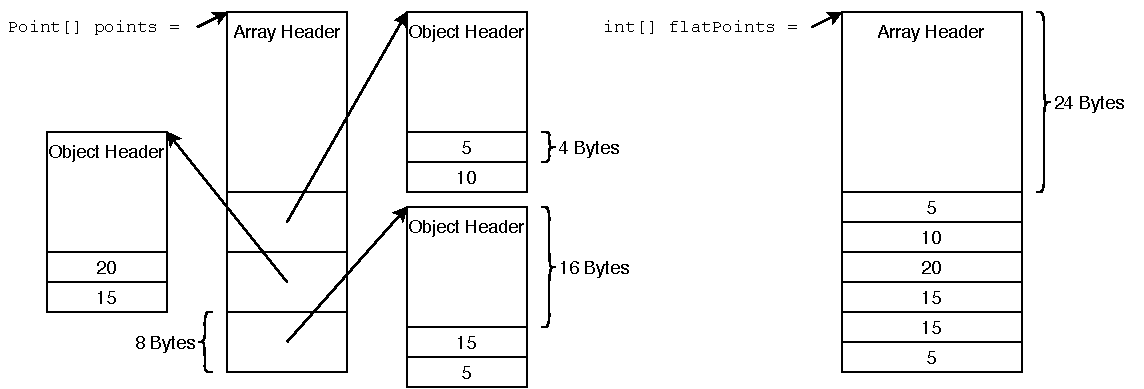
\includegraphics[width=\textwidth]{img/memory-usage.pdf}
    \vspace{-3ex}
    \caption{Vergleich des Speicherlayouts eines Arrays von Punkten (links) und von Zahlen (rechts)}
    \label{fig:memory-usage}
\end{figure}

Hier ist die doppelte Indirektion von der Variable bis zu einem der Punkte durch Verfolgen der Pfeile zu erkennen.
Um anhand der Variable auf einen Koordinate zuzugreifen, werden im schlechtesten Fall zwei Zugriffe auf den Hauptspeicher benötigt, da die Objekte an beliebigen Stellen darin liegen können.
Ebenfalls zu beachten ist der Speicherverbrauch, der sich wie folgt berechnet:

\begin{equation}
    \begin{split}
    \textit{Speicherverbrauch} & = \textit{Array-Header} + 3 \cdot (\textit{Referenz} + \textit{Objekt-Header} + 2 \cdot \textit{int}) \\
    & = \SI{24}{\Byte} + 3 \cdot (\SI{8}{\Byte} + \SI{16}{\Byte} + 2 \cdot \SI{4}{\Byte}) \\
    & = \SI{120}{\Byte}\label{eq:memory-usage-current} \\
    \end{split}
\end{equation}

Eine alternative Implementierung dieses Scenarios kann erfolgen, indem ein Array von \code{int-Werten} verwendet wird.
Dies wird auf der rechten Seite von Abbildung~\ref{fig:memory-usage} dargestellt.
Es fällt auf, dass ohne die zusätzlichen Objekte nicht dur die doppelte Indirektion, sondern auch die Objekt-Header entfallen.
Dadurch ergibt sich ein deutliche kleinerer Speicherverbrauch:

\begin{equation}
    \begin{split}
        \textit{Speicherverbrauch} & = \textit{Array-Header} + 6 * \textit{int} \\
        & = \SI{24}{\Byte} + 6 \cdot \SI{4}{\Byte} \\
        & = \SI{48}{\Byte}\label{eq:memory-usage-flat}
    \end{split}
\end{equation}

Folglich konnten $\SI{72}{\Byte}$ eingespart werden.
Der Effekt wird verstärkt, wenn das Array mehr Elemente enthält.
Zu beachten ist auch, dass die gesamten Daten des Arrays mit einer Größe von $\SI{48}{\Byte}$ in eine Cache-Zeile passen, wenn bei deren Größe von $\SI{64}{\Byte}$ ausgangen wird.

Ein Nachteil dieser Datenmodellierung ist, dass nun der Zugriff auf einzelne Koordinaten erschwert wird.
Statt \code{points[1].y} muss nun \code{flatPoints[3]} verwendet werden, um die y-Koordinate des zweiten Punkts im Array zu erhalten.
Das erschwert den Programmieraufwand und ist fehleranfälliger.
Weiterhin ist es nicht mehr direkt möglich, einen ganzen Punkt aus dem Array zur Weiterverarbeitung zu entnehmen.
Eine optimale Lösung wäre ein Kompromiss zwischen beiden Ansätzen, sodass beim Programmieren ein \code{Point[]} verwendet werden kann, während zur Laufzeit das Speicherlayout wie auf der rechten Seite von Abbildung~\ref{fig:memory-usage} aussieht.

% TODO woanders
%Neben Punkten lassen sich mit Value Types eine Vielzahl von neuen Datentypen definieren, die breite Anwendung finden können.
%Dazu gehören im Bereich der numerischen Datenverarbeitung komplexe, vorzeichenlose und Dezimalzahlen, Binärzahlen größer als 64 bit und Vektoren, die auf modernen \acp{cpu} effizient verarbeitet werden können.
%Auch algebraische Datentypen wie \code{Optional}, \code{Either}, \code{Unit} und Tupel sind wichtige Einsatzmöglichkeiten.
%Letztere benötigen jedoch besondere Sprachunterstützung, die noch nicht Teil des Projekts ist.
